\documentclass[twocolumn,aps,pra,floatfix,amsmath,amssymb,longbibliography]{revtex4-2}

\usepackage[T1]{fontenc}
\usepackage{amsthm}
\usepackage{booktabs}
\usepackage{xcolor}
\usepackage{tikz}
\usetikzlibrary{calc}
\usepackage[
  breaklinks=true,
  colorlinks=true,
  citecolor=black,
  linkcolor=black,
  urlcolor=black
]{hyperref}
\usepackage{orcidlink}

% Highlight passages newly written or substantially rewritten for optional
% editing in the authors' own voice.  To remove all blue highlighting before
% submission, replace `\color{blue}` with nothing (`\newenvironment{handrewrite}{}{}`).
\newenvironment{handrewrite}{\leavevmode\color{blue}}{}
\newcommand{\handrewriteinline}[1]{{\color{blue}#1}}

\newtheorem{theorem}{Theorem}
\newtheorem{lemma}[theorem]{Lemma}
\newtheorem{proposition}[theorem]{Proposition}
\newtheorem{corollary}[theorem]{Corollary}
\theoremstyle{definition}
\newtheorem{definition}[theorem]{Definition}
\newtheorem{example}[theorem]{Example}
\theoremstyle{remark}
\newtheorem{remark}[theorem]{Remark}

\newcommand{\ii}{\mathrm{i}}
\newcommand{\C}{\mathbb C}
\newcommand{\R}{\mathbb R}
\newcommand{\Htwenty}{\mathsf H_{20}}
\newcommand{\Htwentyone}{\mathsf H_{21}}

\definecolor{ctx1}{RGB}{230,25,75}
\definecolor{ctx2}{RGB}{60,180,75}
\definecolor{ctx3}{RGB}{0,130,200}
\definecolor{ctx4}{RGB}{245,130,48}
\definecolor{ctx5}{RGB}{145,30,180}
\definecolor{ctx6}{RGB}{70,240,240}
\definecolor{ctx7}{RGB}{240,50,230}
\definecolor{ctx8}{RGB}{210,245,60}
\definecolor{ctx9}{RGB}{250,190,190}
\definecolor{ctx10}{RGB}{0,128,128}
\definecolor{ctx11}{RGB}{128,128,0}
\definecolor{ctx12}{RGB}{170,110,40}
\definecolor{ctx13}{RGB}{128,0,0}
\definecolor{ctx14}{RGB}{0,0,128}
\tikzset{ctxline/.style={line width=0.95pt,line cap=round}}

\newcommand{\twodotlabel}[5]{%
  \node[circle,fill=#1,draw=#1,minimum size=7.2pt,inner sep=0pt,
        label={[font=\scriptsize,label distance=0.7mm]#3:{#4}}] at #5 {};
  \node[circle,fill=#2,draw=#2,minimum size=4.2pt,inner sep=0pt] at #5 {};
}

\begin{document}

\title{Complex coordinates forced by finite orthogonality hypergraphs in dimension three}

\author{Mirko Navara\,\orcidlink{0000-0002-0880-5992}}
\affiliation{Faculty of Electrical Engineering, Czech Technical University in Prague,
Technick\'{a} 2, CZ-166~27 Prague 6, Czech Republic}
\email{navara@fel.cvut.cz}

\author{Karl Svozil\,\orcidlink{0000-0001-6554-2802}}
\affiliation{Institute for Theoretical Physics, TU Wien,
Wiedner Hauptstra{\ss}e 8-10/136, A-1040 Vienna, Austria}
\email[Corresponding author: ]{karl.svozil@tuwien.ac.at}

\date{\today}

\begin{abstract}
\begin{handrewrite}
In the Cartesian basis of a spin-1 particle, Kochen--Specker squared-spin measurements along orthogonal spatial triads correspond precisely to orthonormal bases in $\R^3$, whose outcomes are unpolarized (spin-nematic) states with zero spin expectation value.  We ask whether every quantum-realizable finite arrangement of overlapping three-outcome projective measurements on a three-level system can be implemented in this purely real way, or whether finite incidence data alone can force complex amplitudes---and hence nonzero spin polarization---in every faithful three-dimensional realization.  First, we establish a general combinatorial obstruction: any three-uniform hypergraph admitting a balanced rational combination of contexts whose residual difference is two disjoint, nonorthogonal vertex pairs forces an equality of two rank-two projector sums and therefore admits no faithful orthogonal representation in $\R^3$.  We realize this criterion with a 20-vertex, 12-context octagonal hypergraph $\Htwenty$ that admits an exact, strictly faithful representation in $\C^3$ (and 26 classical two-valued states), reducing the size of previously known $\C^3$-only hypergraphs by more than half.  Second, to show that the separation persists even when spectral rigidity fails, we augment $\Htwenty$ to a 21-vertex, 14-context hypergraph $\Htwentyone$ in which both inner pairs become orthogonal bases of a common plane; $\Htwentyone$ still admits a clean algebraic representation in $\C^3$ while remaining impossible in $\R^3$ through cyclic Gram closure.  Finally, phase-adjusted realification yields explicit faithful representations of both hypergraphs in $\R^6$, where each triple ceases to be maximal, clarifying how fixed dimension, rank-one outcomes, equivalent pure-state mixtures (pseudocontexts), and spin-1 polarization enter the real-complex distinction.
\end{handrewrite}
\end{abstract}

\maketitle

\section{Introduction}
\label{sec:intro}

\begin{handrewrite}
Kochen and Specker famously realized their theorem on a spin-1 particle by measuring the commuting squared spin components $S_{\mathbf e_1}^2, S_{\mathbf e_2}^2, S_{\mathbf e_3}^2$ along orthogonal spatial triads $\{\mathbf e_1,\mathbf e_2,\mathbf e_3\}\subset\R^3$~\cite{kochen1}.  In the Cartesian basis $\{|x\rangle,|y\rangle,|z\rangle\}$ of a spin-1 system, the eigenstate with zero spin projection along a real unit direction $\mathbf n$ is represented by the real vector $\mathbf n$ itself, and its mean spin vector vanishes ($\langle\mathbf S\rangle=\mathbf 0$).  Any finite family of overlapping squared-spin measurements therefore corresponds directly to a finite collection of real orthonormal bases in $\R^3$.  This raises a simple, concrete question: can every quantum-realizable finite arrangement of overlapping three-outcome projective measurements on a three-level system be implemented using squared-spin measurements alone?  Or do some finite overlap patterns intrinsically demand complex relative phases---meaning that in every faithful three-dimensional quantum realization, regardless of the choice of basis, at least one outcome state must carry nonzero spin polarization?

To make this question precise, we represent a finite measurement arrangement by a three-uniform \emph{orthogonality hypergraph} $\mathsf H=(V,\mathcal E)$: each vertex $v\in V$ labels an elementary rank-one outcome projector, and each three-element hyperedge $E\in\mathcal E$ (a \emph{context}) specifies three mutually exclusive outcomes forming a complete measurement.  A \emph{faithful orthogonal representation}~\cite{lovasz-79,Portillo-2015} in $\mathbb F^3$ ($\mathbb F=\R$ or $\C$) assigns a nonzero vector $x_v\in\mathbb F^3$ to each vertex so that distinct vertices define distinct rays and two rays are orthogonal \emph{if and only if} they belong to a common context.  In particular, neither ray coincidences nor unlisted orthogonalities are permitted.  Notice how this fixed-dimension question fits within the wider debate over real versus complex quantum theory.  If dimension doubling ($\C^n\hookrightarrow\R^{2n}$) is permitted, single-system quantum statistics can be reproduced within a real Hilbert space~\cite{McKague2009SimulatingRealHilbert,Hardy2012LimitedHolism,Aleksandrova2013UniversalQubit}, whereas dimension-independent falsifications of real quantum theory rely on network source independence and tensor-product structure~\cite{renou-2021,Weilenmann2025PartialIndependencePRL} (for operational discrimination tasks, see Ref.~\cite{Bednorz2022OptimalDiscrimination}).  Here we examine a complementary, single-system regime: the Hilbert-space dimension is held fixed at three, each context is required to be a maximal projective measurement, and no entanglement or network assumption enters.

Earlier work established that finite three-uniform hypergraphs can indeed separate $\C^3$ from $\R^3$.  Harding and Salinas Schmeis constructed an orthogonality diagram representable in $\C^3$ but not in $\R^3$~\cite{harding2025remarksIJTP}; counting the two 25-vertex, 16-context gadgets in their Fig.~2 and Theorem~2.6 gives 48 vertices and 32 specified triples once the edge joining their centers is completed to a triple (without imposing our additional exclusion of unlisted orthogonalities).  Similarly, Kochen--Specker (KS) completions built from mutually unbiased bases yield 69-ray, 50-context configurations~\cite{svozil-2025-MYOCHS}.  In this paper we develop a direct algebraic-combinatorial method for forcing complex coordinates at fixed dimension and apply it to obtain two much smaller, exact, strictly faithful constructions---with 20 vertices and 12 contexts ($\Htwenty$) and 21 vertices and 14 contexts ($\Htwentyone$)---each governed by a distinct obstruction to real coordinates and completely independent of KS uncolorability.

Our approach begins in Sec.~\ref{sec:prelim} with a general sufficient criterion for real nonrepresentability (Theorem~\ref{thm:covering-criterion}).  Whenever a balanced rational linear combination of context completeness relations cancels every vertex except two disjoint, nonorthogonal pairs $\{a_1,a_2\}$ and $\{b_1,b_2\}$, every three-dimensional representation must satisfy the projector identity $P_{a_1}+P_{a_2}=P_{b_1}+P_{b_2}$.  Over $\R^3$, the two distinct eigenvalues of a rank-two sum of nonorthogonal projectors fix the pair of rays uniquely (Lemma~\ref{lem:real-rigidity}), contradicting faithfulness; geometrically, an off-center midpoint inside a real Bloch disk determines a single chord, whereas on the complex Bloch sphere an entire circle of chords shares the same midpoint.  The simplest cyclic hypergraph realizing this covering criterion turns out to be an \emph{octagon}: taking an alternating sum of perimeter contexts around a $2k$-gon cancels all corners, and cancelling the midpoints via opposite-midpoint diagonals forces opposite midpoints to carry the same parity, so $k$ must be even; $k=2$ (a square) degenerates to $P_{a_1}=P_{b_1}$, which fails over $\C^3$ as well, leaving $k=4$ as the minimal cyclic skeleton.  In Sec.~\ref{sec:h20} we analyze this 20-vertex octagonal hypergraph $\Htwenty$: nonexistence over $\R^3$ follows immediately from Theorem~\ref{thm:covering-criterion}, while a quarter-turn symmetry ansatz together with cyclic Gram closure produces explicit algebraic coordinates in $\C^3$ whose strict faithfulness we certify across all 190 ray pairs.

Because Theorem~\ref{thm:covering-criterion} relies on nonorthogonality of the two inner pairs, it is natural to ask whether the real-complex obstruction disappears once both pairs are made orthogonal.  In Sec.~\ref{sec:h21} we test this by adding a single vertex $c$ and two contexts $\{a_1,c,a_2\}$ and $\{b_1,c,b_2\}$, obtaining the 21-vertex, 14-context hypergraph $\Htwentyone$.  The projector sum $P_{a_1}+P_{a_2}=P_{b_1}+P_{b_2}=I_{c^\perp}$ then becomes degenerate and poses no obstacle in $\R^3$, yet $\Htwentyone$ still cannot be faithfully represented in $\R^3$: the perimeter Gram-closure equations clash directly with the inner orthogonalities and reduce to a strictly positive quadratic expression.  Over $\C^3$, by contrast, the same symmetry ansatz simplifies at the orthogonal limit to a clean algebraic realization whose 168 unprescribed ray pairs take only two squared overlaps, $1/4$ and $1/2$.

Finally, to pinpoint the exact role of fixed dimension and context maximality, Sec.~\ref{sec:realification} applies phase-adjusted realification~\cite{svozil-2025-rvc} to construct explicit faithful real representations of both $\Htwenty$ and $\Htwentyone$ in $\R^6$, where each specified triple spans only a three-dimensional subspace and ceases to be maximal.  Section~\ref{sec:physical} develops the physical implications for spin-1 polarization, equivalent pure-state mixtures (pseudocontexts~\cite{2026-Navara-Svozil-pseudocontexts}), and prospective fixed-dimension tests, and Sec.~\ref{sec:discussion} compares the two algebraic mechanisms, classical state-separation properties, and connections to the contextuality literature before we conclude in Sec.~\ref{sec:conclusion}.
\end{handrewrite}

\section{Orthogonality representations, algebraic lemmas, and a covering criterion}
\label{sec:prelim}

Throughout, we use the physics convention for the Hermitian inner product,
which is conjugate-linear in the first argument:
\begin{equation}
 \langle x,y\rangle=\sum_{k=1}^{d}\overline{x_k}\,y_k.
 \label{eq:inner-product}
\end{equation}

\begin{definition}
\label{def:for}
Let $\mathsf H=(V,\mathcal E)$ be a three-uniform hypergraph, let
$\mathbb F$ be either $\R$ or $\C$, and let $d\ge3$.
Hyperedges are unordered three-element subsets of $V$, and no hyperedge
is repeated.  A \emph{faithful orthogonal representation} of $\mathsf H$ in
$\mathbb F^d$ assigns a nonzero vector $x_v\in\mathbb F^d$ to every $v\in V$
such that:
\begin{enumerate}
\item distinct vertices determine distinct rays; and
\item $\langle x_u,x_v\rangle=0$ if and only if $u$ and $v$ belong to a
common hyperedge.
\end{enumerate}
Each hyperedge is then an orthogonal triple.  For $d=3$ it is an orthogonal
basis and hence a maximal \emph{context}; for $d>3$ the same specified triple
need not be maximal.
\end{definition}

For any nonzero column vector $x$, let $x^\dagger$ denote its conjugate
transpose and write
\begin{equation}
 P_x=\frac{xx^\dagger}{\langle x,x\rangle}
 \label{eq:projector}
\end{equation}
for the rank-one projector onto its ray $[x]$.  Because $P_x$ is invariant
under nonzero rescaling of $x$, any ray may be represented by an unnormalized
nonzero vector without changing its projector.  In a three-dimensional
representation, a context $\{x,y,z\}$ satisfies
\begin{equation}
 P_x+P_y+P_z=I_3.
 \label{eq:context-sum}
\end{equation}
Consequently, linear combinations of three-dimensional context equations can
force projector identities that hold in every representation of the hypergraph
in that dimension.

For $x,y\in\C^3$ define the Hermitian cross product by
\begin{equation}
 x\boxtimes y:=\overline{x\times y},
 \label{eq:hcross}
\end{equation}
where $x\times y$ is the ordinary bilinear cross product.  Then
$x\boxtimes y$ is Hermitian-orthogonal to both $x$ and $y$.

\begin{lemma}[Cyclic Gram closure]
\label{lem:gram-closure}
Let $x,y,z\in\C^3$, and suppose $x\boxtimes y$ and
$y\boxtimes z$ are nonzero.  Then
\begin{equation}
 \langle x\boxtimes y,y\boxtimes z\rangle=0
 \quad\Longleftrightarrow\quad
 \langle x,y\rangle\langle y,z\rangle
 =\langle x,z\rangle\langle y,y\rangle.
 \label{eq:gram-closure}
\end{equation}
\end{lemma}

\begin{proof}
The bilinear Lagrange identity, with $\mathbin{\cdot}$ denoting the standard
bilinear dot product on $\C^3$, gives
\[
 (x\times y)\mathbin{\cdot}(\bar y\times\bar z)
 =(x\mathbin{\cdot}\bar y)(y\mathbin{\cdot}\bar z)
 -(x\mathbin{\cdot}\bar z)(y\mathbin{\cdot}\bar y).
\]
Indeed, for arbitrary $u,w\in\C^3$,
$\langle\bar u,\bar w\rangle=u\mathbin{\cdot}\bar w$; taking
$u=x\times y$ and $w=y\times z$ therefore identifies the left-hand side
with $\langle x\boxtimes y,y\boxtimes z\rangle$.  The right-hand side
is the complex conjugate of
\[
 \langle x,y\rangle\langle y,z\rangle
 -\langle x,z\rangle\langle y,y\rangle.
\]
Their vanishing is therefore equivalent.
\end{proof}

\begin{lemma}[Rigidity of two real rays]
\label{lem:real-rigidity}
Let $u_1,u_2,w_1,w_2\in\R^3\setminus\{0\}$ be nonzero real vectors satisfying
\begin{equation}
 P_{u_1}+P_{u_2}=P_{w_1}+P_{w_2}.
 \label{eq:two-sums}
\end{equation}
If $u_1$ and $u_2$ represent distinct, nonorthogonal rays, then
$\{[w_1],[w_2]\}=\{[u_1],[u_2]\}$ as unordered pairs of rays.
\end{lemma}

\begin{proof}
Because $P_x$ is invariant under nonzero rescaling, we may normalize all four
vectors to unit length.  All four vectors lie in the range of the common
operator in Eq.~\eqref{eq:two-sums}.  Choose signs so that
$\gamma=\langle u_1,u_2\rangle\in(0,1)$.  The two nonzero eigenvalues
are $1+\gamma$ and $1-\gamma$, with eigenvectors $u_1+u_2$ and
$u_1-u_2$, respectively.  Choose signs and order for $w_1,w_2$ so
that $\delta=\langle w_1,w_2\rangle\ge0$.  The common operator has rank two,
so $\delta<1$.  Equality of spectra gives
$\delta=\gamma$.  Since the two eigenvalues are distinct, there are real
nonzero scalars $\lambda,\mu$ such that
\[
 w_1+w_2=\lambda(u_1+u_2),\qquad
 w_1-w_2=\mu(u_1-u_2).
\]
Comparing squared norms on both sides yields
\begin{align*}
 \lambda^2(1+\gamma)+\mu^2(1-\gamma)&=2,\\
 \lambda^2(1+\gamma)-\mu^2(1-\gamma)&=2\gamma.
\end{align*}
Hence $\lambda^2=\mu^2=1$.  Solving for $w_1,w_2$ recovers the two
original rays, possibly with signs and permutation.
\end{proof}

\begin{handrewrite}
Notice why Lemma~\ref{lem:real-rigidity} fails over $\C^3$: in complex vector
space, the corresponding eigenvalue equations constrain only $|\lambda|^2=|\mu|^2=1$,
leaving an arbitrary relative phase $\eta=\mu/\lambda\in S^1$ between the two
eigenvectors.  Whenever $\eta\notin\{1,-1\}$, the resulting pair
$[w_1],[w_2]$ is disjoint from $[u_1],[u_2]$ yet generates the exact same
projector sum.  Combining Lemma~\ref{lem:real-rigidity} with the context
completeness relation~\eqref{eq:context-sum} yields a general combinatorial
obstruction to real three-dimensional representability.
\end{handrewrite}

\begin{theorem}[Balanced covering obstruction over $\R^3$]
\label{thm:covering-criterion}
Let $\mathsf H=(V,\mathcal E)$ be a three-uniform hypergraph.  Suppose there
exist rational weights $c_E\in\mathbb Q$ ($E\in\mathcal E$) and four distinct
vertices $a_1,a_2,b_1,b_2\in V$, with $a_1$ and $a_2$ belonging to no common
hyperedge, such that for every vertex $v\in V$,
\begin{equation}
 \sum_{\substack{E\in\mathcal E\\ v\in E}} c_E
 =\delta_{v,a_1}+\delta_{v,a_2}-\delta_{v,b_1}-\delta_{v,b_2}.
 \label{eq:covering-criterion}
\end{equation}
Then $\mathsf H$ admits no faithful orthogonal representation in $\R^3$.
\end{theorem}

\begin{proof}
Because every hyperedge has cardinality three, summing
Eq.~\eqref{eq:covering-criterion} over all $v\in V$ gives
\[
 3\sum_{E\in\mathcal E} c_E
 =\sum_{v\in V}\sum_{\substack{E\in\mathcal E\\ v\in E}} c_E
 =1+1-1-1=0,
\]
so $\sum_{E\in\mathcal E} c_E=0$ automatically.  Suppose for contradiction
that $\{x_v\}_{v\in V}\subset\R^3\setminus\{0\}$ is a faithful orthogonal
representation of $\mathsf H$.  Multiplying the completeness identity
$\sum_{v\in E} P_{x_v}=I_3$ by $c_E$ and summing over $E\in\mathcal E$ yields
\begin{align*}
 P_{x_{a_1}}+P_{x_{a_2}}-P_{x_{b_1}}-P_{x_{b_2}}
 &=\sum_{v\in V}\!\left(\sum_{\substack{E\in\mathcal E\\ v\in E}} c_E\right)P_{x_v}\\
 &=\sum_{E\in\mathcal E} c_E\sum_{v\in E} P_{x_v}\\
 &=\left(\sum_{E\in\mathcal E} c_E\right)I_3=0,
\end{align*}
and therefore $P_{x_{a_1}}+P_{x_{a_2}}=P_{x_{b_1}}+P_{x_{b_2}}$.
By faithfulness, since $a_1$ and $a_2$ are distinct and share no hyperedge,
the real vectors $x_{a_1}$ and $x_{a_2}$ represent distinct, nonorthogonal
rays.  Lemma~\ref{lem:real-rigidity} then forces
$\{[x_{b_1}],[x_{b_2}]\}=\{[x_{a_1}],[x_{a_2}]\}$, contradicting the
requirement that the four distinct vertices $a_1,a_2,b_1,b_2$ label four
distinct rays.
\end{proof}

\begin{handrewrite}
In the terminology of Ref.~\cite{2026-Navara-Svozil-pseudocontexts},
Eq.~\eqref{eq:covering-criterion} certifies that $\{a_1,a_2\}$ and
$\{b_1,b_2\}$ form a pair of size-two \emph{pseudocontexts} whose summed
probabilities must coincide in every admissible weight.
Theorem~\ref{thm:covering-criterion} shows that any such combinatorial
certificate immediately rules out $\R^3$ realizations while leaving open
faithful complex realizations in $\C^3$.
\end{handrewrite}

\section{The 20-ray octagon}
\label{sec:h20}

\subsection{Minimal cyclic covering and nonexistence over
\texorpdfstring{$\R^3$}{R3}}

\begin{handrewrite}
To realize Theorem~\ref{thm:covering-criterion} with the simplest cyclic
architecture, consider a $2k$-gon of perimeter contexts
$E_j=\{v_{j-1,j},v_j,v_{j,j+1}\}$ ($j\in\mathbb Z_{2k}$) and assign
alternating weights $+1$ to odd $j$ and $-1$ to even $j$.  Every corner
vertex $v_{j,j+1}$ belongs to one odd and one even perimeter context, so all
corner contributions cancel.  To cancel the $2k$ midpoint vertices by adding
$k$ inner contexts $D_j=\{v_j,u_j,v_{j+k}\}$ joining opposite midpoints,
opposite indices $j$ and $j+k$ must have the same parity, which requires $k$
to be even.  For $k=2$ (a square), the residual difference reduces to a
single vertex on each side, forcing $P_{a_1}=P_{b_1}$ and hence
$[a_1]=[b_1]$ over \emph{both} $\R^3$ and $\C^3$.  The smallest even value
producing a two-versus-two residual difference is therefore $k=4$---an
\emph{octagon}.
\end{handrewrite}

Accordingly, the vertices of $\Htwenty$ are eight midpoint vertices
$v_0,\ldots,v_7$, eight corner vertices
$v_{01},v_{12},\ldots,v_{70}$, and four inner vertices
$a_1,a_2,b_1,b_2$, with indices read modulo eight.  The eight perimeter
contexts and four inner contexts are
\begin{align}
 E_j&=\{v_{j-1,j},v_j,v_{j,j+1}\}, &&j=0,\ldots,7,
 \label{eq:perimeter-contexts}\\
 D_0&=\{v_0,a_1,v_4\},&D_2&=\{v_2,a_2,v_6\},\nonumber\\
 D_1&=\{v_1,b_2,v_5\},&D_3&=\{v_3,b_1,v_7\}.
 \label{eq:inner-contexts}
\end{align}
The incidence structure is shown in Fig.~\ref{fig:h20}, and
Table~\ref{tab:contexts} lists all contexts of both octagons studied in this
paper.

\begin{figure*}[t]
\centering
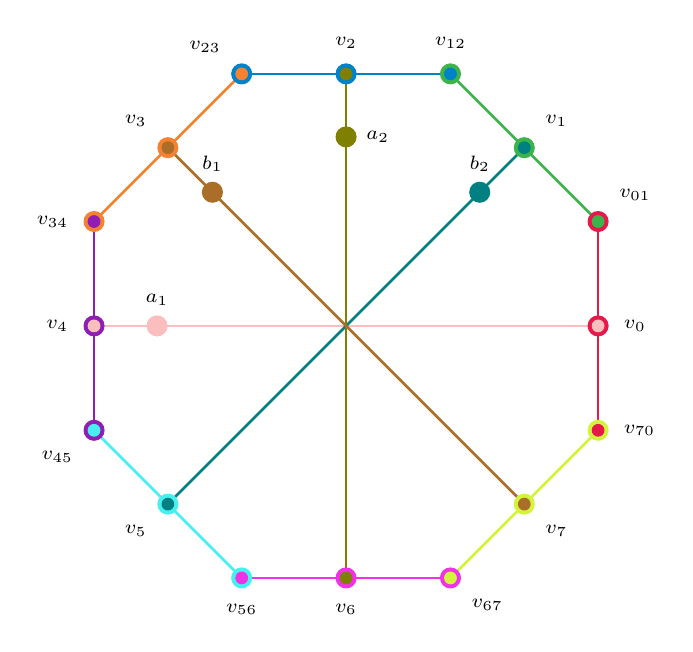
\begin{tikzpicture}[scale=1.6,every label/.style={font=\scriptsize}]
  \def\Rmid{2}
  \def\Rcor{2.1648}%
  \def\Rinn{1.5}
  \foreach \i/\j/\ang in {
    0/1/22.5,1/2/67.5,2/3/112.5,3/4/157.5,
    4/5/202.5,5/6/247.5,6/7/292.5,7/0/337.5
  }{\coordinate (v\i\j) at (\ang:\Rcor);}
  \foreach \i/\ang in {
    0/0,1/45,2/90,3/135,4/180,5/225,6/270,7/315
  }{\coordinate (v\i) at (\ang:\Rmid);}
  \coordinate (a1) at (180:\Rinn);
  \coordinate (a2) at (90:\Rinn);
  \coordinate (b1) at (135:\Rinn);
  \coordinate (b2) at (45:\Rinn);

  \draw[ctxline,draw=ctx1] (v70)--(v01);
  \draw[ctxline,draw=ctx2] (v01)--(v12);
  \draw[ctxline,draw=ctx3] (v12)--(v23);
  \draw[ctxline,draw=ctx4] (v23)--(v34);
  \draw[ctxline,draw=ctx5] (v34)--(v45);
  \draw[ctxline,draw=ctx6] (v45)--(v56);
  \draw[ctxline,draw=ctx7] (v56)--(v67);
  \draw[ctxline,draw=ctx8] (v67)--(v70);
  \draw[ctxline,draw=ctx9] (v0)--(v4);
  \draw[ctxline,draw=ctx10] (v1)--(v5);
  \draw[ctxline,draw=ctx11] (v2)--(v6);
  \draw[ctxline,draw=ctx12] (v3)--(v7);

  \twodotlabel{ctx1}{ctx2}{above right}{$v_{01}$}{(v01)}
  \twodotlabel{ctx2}{ctx3}{above}{$v_{12}$}{(v12)}
  \twodotlabel{ctx3}{ctx4}{above left}{$v_{23}$}{(v23)}
  \twodotlabel{ctx4}{ctx5}{left}{$v_{34}$}{(v34)}
  \twodotlabel{ctx5}{ctx6}{below left}{$v_{45}$}{(v45)}
  \twodotlabel{ctx6}{ctx7}{below}{$v_{56}$}{(v56)}
  \twodotlabel{ctx7}{ctx8}{below right}{$v_{67}$}{(v67)}
  \twodotlabel{ctx8}{ctx1}{right}{$v_{70}$}{(v70)}
  \twodotlabel{ctx1}{ctx9}{right}{$v_0$}{(v0)}
  \twodotlabel{ctx2}{ctx10}{above right}{$v_1$}{(v1)}
  \twodotlabel{ctx3}{ctx11}{above}{$v_2$}{(v2)}
  \twodotlabel{ctx4}{ctx12}{above left}{$v_3$}{(v3)}
  \twodotlabel{ctx5}{ctx9}{left}{$v_4$}{(v4)}
  \twodotlabel{ctx6}{ctx10}{below left}{$v_5$}{(v5)}
  \twodotlabel{ctx7}{ctx11}{below}{$v_6$}{(v6)}
  \twodotlabel{ctx8}{ctx12}{below right}{$v_7$}{(v7)}
  \node[circle,fill=ctx9,draw=ctx9,minimum size=7.2pt,inner sep=0pt,
        label={[font=\scriptsize]above:{$a_1$}}] at (a1) {};
  \node[circle,fill=ctx11,draw=ctx11,minimum size=7.2pt,inner sep=0pt,
        label={[font=\scriptsize]right:{$a_2$}}] at (a2) {};
  \node[circle,fill=ctx12,draw=ctx12,minimum size=7.2pt,inner sep=0pt,
        label={[font=\scriptsize]above:{$b_1$}}] at (b1) {};
  \node[circle,fill=ctx10,draw=ctx10,minimum size=7.2pt,inner sep=0pt,
        label={[font=\scriptsize]above:{$b_2$}}] at (b2) {};
\end{tikzpicture}
\caption{The 20-ray hypergraph $\Htwenty$.  The eight perimeter contexts
$E_0,\ldots,E_7$ form the octagon; the four inner contexts join opposite
midpoints through $a_1,a_2,b_1,b_2$.  Each color denotes one context.}
\label{fig:h20}
\end{figure*}

\begin{table}[tb]
\caption{The twelve contexts of $\Htwenty$ and the two additional
contexts of $\Htwentyone$.  All fourteen contexts belong to $\Htwentyone$;
only $F_a$ and $F_b$ are absent from $\Htwenty$.}
\label{tab:contexts}
\centering
\begin{tabular}{@{}ll@{}}
\toprule
Context & Vertices (unordered) \\
\midrule
$E_0$ & $\{v_{70},v_0,v_{01}\}$ \\
$E_1$ & $\{v_{01},v_1,v_{12}\}$ \\
$E_2$ & $\{v_{12},v_2,v_{23}\}$ \\
$E_3$ & $\{v_{23},v_3,v_{34}\}$ \\
$E_4$ & $\{v_{34},v_4,v_{45}\}$ \\
$E_5$ & $\{v_{45},v_5,v_{56}\}$ \\
$E_6$ & $\{v_{56},v_6,v_{67}\}$ \\
$E_7$ & $\{v_{67},v_7,v_{70}\}$ \\
\midrule
$D_0$ & $\{v_0,a_1,v_4\}$ \\
$D_1$ & $\{v_1,b_2,v_5\}$ \\
$D_2$ & $\{v_2,a_2,v_6\}$ \\
$D_3$ & $\{v_3,b_1,v_7\}$ \\
\midrule
$F_a$ & $\{a_1,c,a_2\}$ \\
$F_b$ & $\{b_1,c,b_2\}$ \\
\bottomrule
\end{tabular}
\end{table}

Partition the twelve contexts of $\Htwenty$ into two complementary
collections of six contexts:
\begin{align*}
 \mathcal A&=\{D_0,D_2,E_1,E_3,E_5,E_7\},\\
 \mathcal B&=\{D_1,D_3,E_0,E_2,E_4,E_6\}.
\end{align*}
Every midpoint and every corner occurs exactly once in $\mathcal A$ and
exactly once in $\mathcal B$; only $a_1,a_2$ occur in $\mathcal A$, and only
$b_1,b_2$ occur in $\mathcal B$.  Setting $c_E=+1$ for $E\in\mathcal A$ and
$c_E=-1$ for $E\in\mathcal B$ therefore satisfies
Eq.~\eqref{eq:covering-criterion} and forces the covering identity
\begin{equation}
 P_{a_1}+P_{a_2}=P_{b_1}+P_{b_2}
 \label{eq:covering-identity}
\end{equation}
in every real or complex three-dimensional representation of $\Htwenty$.
Because $a_1$ and $a_2$ belong to no common context of $\Htwenty$,
Theorem~\ref{thm:covering-criterion} yields immediately:

\begin{corollary}
\label{cor:h20-real}
The hypergraph $\Htwenty$ has no faithful orthogonal representation in
$\R^3$.
\end{corollary}

\subsection{Construction of an exact faithful representation over
\texorpdfstring{$\C^3$}{C3}}

\begin{handrewrite}
To show that $\Htwenty$ is genuinely representable over $\C^3$ rather than
overconstrained over both fields, we construct its coordinates systematically
from the covering identity~\eqref{eq:covering-identity} and cyclic Gram
closure.  Choose a basis of $\C^3$ in which the common rank-two operator
$P_{a_1}+P_{a_2}=P_{b_1}+P_{b_2}$ is diagonal on the $xy$-plane with nonzero
eigenvalues proportional to $(C,1)$ for a real parameter $0<C<1$.  Setting
$s=\sqrt C$ and $N=1+C$, the complex phase freedom remarked after
Lemma~\ref{lem:real-rigidity} yields the four unnormalized ray
representatives $a_{1,2}=(s,\pm1,0)$ and $b_{1,2}=(s,\pm\eta,0)$ for any unit
phase $\eta\notin\{1,-1\}$.  Orthogonality to the inner rays and antipodal
orthogonality $\langle v_j,v_{j+4}\rangle=0$ then constrain the eight
midpoints to the form $v_j=(1,s\mu_j,r\tau_j)$ with $r=\sqrt N$,
$\mu_{j+4}=\mu_j$, and $\tau_{j+4}=-\tau_j$.  Imposing the quarter-turn
symmetry $\mu_{j+2}=-\mu_j$ and $\tau_{j+2}=-\ii\tau_j$ collapses all eight
perimeter closure relations~\eqref{eq:gram-closure} to a single complex
equation linking $C$, $\eta$, and the single remaining unit phase
$\zeta=\tau_1$.  Choosing the rational Pythagorean phase
$\eta=(5+12\ii)/13$ makes the real and imaginary parts of that closure
equation linear in $\zeta=x+\ii y$; solving for $(x,y)$ in terms of $C$ and
imposing the unit-circle condition $x^2+y^2=1$ produces a quadratic equation
for $C$ whose smaller positive root gives the closed-form solution below.
\end{handrewrite}

Explicitly, set
\begin{equation}
 \begin{aligned}
 C&=\frac{49-5\sqrt{69}}{26},&s&=\sqrt C,\\
 N&=1+C,&r&=\sqrt N.
 \end{aligned}
 \label{eq:C-definition}
\end{equation}
The number $C$ is the smaller positive root of
\begin{equation}
 13C^2-49C+13=0,
 \label{eq:C-polynomial}
\end{equation}
so $0<C<1$.  Define the unit phases
\begin{align}
 \eta&=\frac{5+12\ii}{13},\label{eq:eta}\\
 \zeta&=\frac{14+6\sqrt{69}}{65}
 +\ii\frac{4\sqrt{69}-21}{65}.
 \label{eq:zeta}
\end{align}
Let
\begin{align*}
 (\mu_0,\ldots,\mu_7)&=(-1,\eta,1,-\eta,-1,\eta,1,-\eta),\\
 (\tau_0,\ldots,\tau_7)&=(1,\zeta,-\ii,-\ii\zeta,
 -1,-\zeta,\ii,\ii\zeta).
\end{align*}
The inner and midpoint rays are represented by the (unnormalized, complex)
vectors
\begin{align}
 a_1&=(s,1,0),&a_2&=(s,-1,0),\nonumber\\
 b_1&=(s,\eta,0),&b_2&=(s,-\eta,0),
 \label{eq:h20-inner-vectors}\\
 v_j&=(1,s\mu_j,r\tau_j),&&j=0,\ldots,7.
 \label{eq:h20-midpoints}
\end{align}
For $j$ modulo eight, define the corner representatives by
\begin{equation}
 v_{j,j+1}=v_j\boxtimes v_{j+1}.
 \label{eq:h20-corners}
\end{equation}
Equivalently, Eq.~\eqref{eq:h20-corners} is the explicit formula
\begin{multline}
 v_{j,j+1}=\bigl(
 sr(\bar\mu_j\bar\tau_{j+1}-\bar\tau_j\bar\mu_{j+1}),\\
 r(\bar\tau_j-\bar\tau_{j+1}),
 s(\bar\mu_{j+1}-\bar\mu_j)\bigr).
 \label{eq:h20-corner-formula}
\end{multline}

\begin{theorem}
\label{thm:h20-complex}
Equations~\eqref{eq:C-definition}--\eqref{eq:h20-corner-formula}
give a faithful orthogonal representation of $\Htwenty$ in $\C^3$.
\end{theorem}

\begin{proof}
First, $|\eta|=1$.  Write $\zeta=x+\ii y$.  The four inner contexts
follow directly from $r^2=N$, $|\eta|=|\zeta|=1$, and the antipodal
relations $\mu_{j+4}=\mu_j$, $\tau_{j+4}=-\tau_j$.  For example,
\[
 \langle a_1,v_0\rangle=0,\qquad
 \langle v_0,v_4\rangle=1+C-r^2=0,
\]
and
\[
 \langle b_2,v_1\rangle=0,\qquad
 \langle v_1,v_5\rangle=1+C-r^2|\zeta|^2=0.
\]
The other two inner contexts are identical calculations.

By construction, $v_{j,j+1}$ is orthogonal to $v_j$ and $v_{j+1}$.
It remains to prove orthogonality of the two corner rays in every
perimeter context.  Put
\[
 G_{jk}=\langle v_j,v_k\rangle
 =1+C\bar\mu_j\mu_k+N\bar\tau_j\tau_k.
\]
Lemma~\ref{lem:gram-closure} reduces the eight remaining conditions to
\begin{equation}
 G_{j-1,j}G_{j,j+1}=G_{j-1,j+1}G_{j,j},
 \qquad j=0,\ldots,7.
 \label{eq:h20-closure}
\end{equation}
Substituting the cyclic patterns for $\mu_j$ and $\tau_j$ reduces all eight
conditions to common real and imaginary equations once $x^2+y^2=1$.
Separating those parts gives
\begin{align}
 7Cx-17Cy-13C-13x+13y+13&=0,
 \label{eq:closure-real}
\end{align}
and
\begin{multline}
 -7C^2x+17C^2y+13C^2-20Cx+30Cy\\
 {}+2C-13x+13y+13=0.
 \label{eq:closure-imag}
\end{multline}
Solving these two linear equations for $x$ and $y$ gives
\begin{equation}
 x=\frac{104-76C}{65(1+C)},\qquad
 y=\frac{39-81C}{65(1+C)}.
 \label{eq:xy-C}
\end{equation}
For these values,
\begin{equation}
 x^2+y^2-1=
 \frac{48(13C^2-49C+13)}{325(1+C)^2}=0.
 \label{eq:zeta-unit}
\end{equation}
Using the smaller root in Eq.~\eqref{eq:C-polynomial},
Eq.~\eqref{eq:xy-C} is exactly the phase in Eq.~\eqref{eq:zeta}.
Thus all twelve triples are contexts.

It remains to exclude unintended orthogonalities and ray coincidences.
The exact overlap certificate in Appendix~\ref{app:faithfulness} shows
that the 36 prescribed unordered pairs have zero overlap, whereas the
154 unprescribed pairs have squared normalized overlaps between $1/25$
and $4/5$.  Hence every unprescribed inner product is nonzero and no two
displayed vectors are proportional.  The representation is faithful.
\end{proof}

As designed, the two complex inner pairs decompose the same rank-two
operator.  Since all four vectors in Eq.~\eqref{eq:h20-inner-vectors} have
squared norm $N$ and $|\eta|=1$,
\begin{equation}
 P_{a_1}+P_{a_2}=P_{b_1}+P_{b_2}
 =\frac{2}{N}\operatorname{diag}(C,1,0).
 \label{eq:complex-two-sum}
\end{equation}
Their within-pair inner products are $C-1\ne0$, and the four rays are
distinct because $\eta\notin\{1,-1\}$.

\section{The 21-ray orthogonal augmentation}
\label{sec:h21}

\begin{handrewrite}
Theorem~\ref{thm:covering-criterion} relies essentially on the nonorthogonality
of $a_1$ and $a_2$, which keeps the two nonzero eigenvalues of
$P_{a_1}+P_{a_2}$ distinct.  Does the octagonal skeleton lose its ability to
separate $\C^3$ from $\R^3$ once that spectral rigidity is removed?  To test
this, we add one vertex $c$ and two contexts
\begin{equation}
 F_a=\{a_1,c,a_2\},\qquad F_b=\{b_1,c,b_2\}
 \label{eq:added-contexts}
\end{equation}
to $\Htwenty$, forming the 21-vertex, 14-context hypergraph $\Htwentyone$
shown in Fig.~\ref{fig:h21}.  The added contexts force both inner pairs to be
orthogonal bases of the same plane $c^\perp$, so the covering identity
collapses to the degenerate relation $P_{a_1}+P_{a_2}=P_{b_1}+P_{b_2}=I_{c^\perp}$,
which poses no obstruction in $\R^3$.  Nevertheless, $\Htwentyone$ still
separates $\C^3$ from $\R^3$: over $\C^3$, the very same quarter-turn ansatz
used in Sec.~\ref{sec:h20} specializes cleanly to the orthogonal limit $C=1$,
$\eta=\ii$, whereas over $\R^3$ the perimeter Gram-closure conditions clash
with the inner orthogonalities.
\end{handrewrite}

\begin{figure*}[t]
\centering
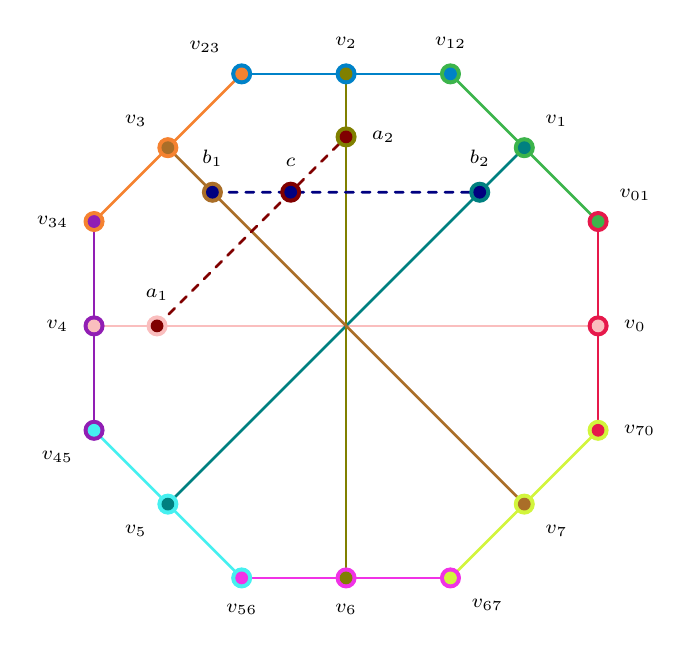
\begin{tikzpicture}[scale=1.6,every label/.style={font=\scriptsize}]
  \def\Rmid{2}
  \def\Rcor{2.1648}%
  \def\Rinn{1.5}
  \foreach \i/\j/\ang in {
    0/1/22.5,1/2/67.5,2/3/112.5,3/4/157.5,
    4/5/202.5,5/6/247.5,6/7/292.5,7/0/337.5
  }{\coordinate (v\i\j) at (\ang:\Rcor);}
  \foreach \i/\ang in {
    0/0,1/45,2/90,3/135,4/180,5/225,6/270,7/315
  }{\coordinate (v\i) at (\ang:\Rmid);}
  \coordinate (a1) at (180:\Rinn);
  \coordinate (a2) at (90:\Rinn);
  \coordinate (b1) at (135:\Rinn);
  \coordinate (b2) at (45:\Rinn);
  \coordinate (c) at ($(a1)!0.70710678!(a2)$);

  \draw[ctxline,draw=ctx1] (v70)--(v01);
  \draw[ctxline,draw=ctx2] (v01)--(v12);
  \draw[ctxline,draw=ctx3] (v12)--(v23);
  \draw[ctxline,draw=ctx4] (v23)--(v34);
  \draw[ctxline,draw=ctx5] (v34)--(v45);
  \draw[ctxline,draw=ctx6] (v45)--(v56);
  \draw[ctxline,draw=ctx7] (v56)--(v67);
  \draw[ctxline,draw=ctx8] (v67)--(v70);
  \draw[ctxline,draw=ctx9] (v0)--(v4);
  \draw[ctxline,draw=ctx10] (v1)--(v5);
  \draw[ctxline,draw=ctx11] (v2)--(v6);
  \draw[ctxline,draw=ctx12] (v3)--(v7);
  \draw[ctxline,dashed,draw=ctx13] (a1)--(c)--(a2);
  \draw[ctxline,dashed,draw=ctx14] (b1)--(c)--(b2);

  \twodotlabel{ctx1}{ctx2}{above right}{$v_{01}$}{(v01)}
  \twodotlabel{ctx2}{ctx3}{above}{$v_{12}$}{(v12)}
  \twodotlabel{ctx3}{ctx4}{above left}{$v_{23}$}{(v23)}
  \twodotlabel{ctx4}{ctx5}{left}{$v_{34}$}{(v34)}
  \twodotlabel{ctx5}{ctx6}{below left}{$v_{45}$}{(v45)}
  \twodotlabel{ctx6}{ctx7}{below}{$v_{56}$}{(v56)}
  \twodotlabel{ctx7}{ctx8}{below right}{$v_{67}$}{(v67)}
  \twodotlabel{ctx8}{ctx1}{right}{$v_{70}$}{(v70)}
  \twodotlabel{ctx1}{ctx9}{right}{$v_0$}{(v0)}
  \twodotlabel{ctx2}{ctx10}{above right}{$v_1$}{(v1)}
  \twodotlabel{ctx3}{ctx11}{above}{$v_2$}{(v2)}
  \twodotlabel{ctx4}{ctx12}{above left}{$v_3$}{(v3)}
  \twodotlabel{ctx5}{ctx9}{left}{$v_4$}{(v4)}
  \twodotlabel{ctx6}{ctx10}{below left}{$v_5$}{(v5)}
  \twodotlabel{ctx7}{ctx11}{below}{$v_6$}{(v6)}
  \twodotlabel{ctx8}{ctx12}{below right}{$v_7$}{(v7)}
  \twodotlabel{ctx9}{ctx13}{above}{$a_1$}{(a1)}
  \twodotlabel{ctx11}{ctx13}{right}{$a_2$}{(a2)}
  \twodotlabel{ctx12}{ctx14}{above}{$b_1$}{(b1)}
  \twodotlabel{ctx10}{ctx14}{above}{$b_2$}{(b2)}
  \twodotlabel{ctx13}{ctx14}{above}{$c$}{(c)}
\end{tikzpicture}
\caption{The 21-ray hypergraph $\Htwentyone$.  The twelve solid contexts
are those of $\Htwenty$; the two dashed contexts meet at the new vertex
$c$.}
\label{fig:h21}
\end{figure*}

\subsection{Exact coordinates over \texorpdfstring{$\C^3$}{C3}}

Setting $C=1$ ($s=1$, $r=\sqrt2$) and $\eta=\ii$ in the quarter-turn
symmetry ansatz of Sec.~\ref{sec:h20}, let
\begin{equation}
 p=\frac{\sqrt{14}+\sqrt2}{4},\qquad
 q=\frac{\sqrt{14}-\sqrt2}{4}.
 \label{eq:pq}
\end{equation}
Then
\begin{equation}
 p^2+q^2=2,\qquad pq=\frac34,\qquad p-q=\frac{\sqrt2}{2}.
 \label{eq:pq-identities}
\end{equation}
Choose the unnormalized complex representatives
\begin{align}
 c&=(0,0,1),\nonumber\\
 a_1&=(1,1,0),&a_2&=(1,-1,0),\nonumber\\
 b_1&=(1,\ii,0),&b_2&=(1,-\ii,0),
 \label{eq:h21-inner}
\end{align}
and the eight midpoint representatives
\begin{align}
 v_0&=(1,-1,\sqrt2),&v_4&=(1,-1,-\sqrt2),\nonumber\\
 v_1&=(1,\ii,p+\ii q),&v_5&=(1,\ii,-p-\ii q),\nonumber\\
 v_2&=(1,1,-\ii\sqrt2),&v_6&=(1,1,\ii\sqrt2),\nonumber\\
 v_3&=(1,-\ii,q-\ii p),&v_7&=(1,-\ii,-q+\ii p).
 \label{eq:h21-midpoints}
\end{align}
The eight corner representatives are
\begin{align}
 v_{01}&=(-p+\ii(q+\sqrt2),\ \sqrt2-p+\ii q,\ 1-\ii),\nonumber\\
 v_{12}&=(\sqrt2-p+\ii q,\ p-\ii(q+\sqrt2),\ 1+\ii),\nonumber\\
 v_{23}&=(q+\sqrt2+\ii p,\ -q+\ii(\sqrt2-p),\ -1+\ii),\nonumber\\
 v_{34}&=(q+\ii(p-\sqrt2),\ q+\sqrt2+\ii p,\ -1-\ii),\nonumber\\
 v_{45}&=(p-\ii(q+\sqrt2),\ -\sqrt2+p-\ii q,\ 1-\ii),\nonumber\\
 v_{56}&=(-\sqrt2+p-\ii q,\ -p+\ii(q+\sqrt2),\ 1+\ii),\nonumber\\
 v_{67}&=(-q-\sqrt2-\ii p,\ q-\ii(\sqrt2-p),\ -1+\ii),\nonumber\\
 v_{70}&=(-q-\ii(p-\sqrt2),\ -q-\sqrt2-\ii p,\ -1-\ii).
 \label{eq:h21-corners}
\end{align}

\begin{theorem}
\label{thm:h21-complex}
Equations~\eqref{eq:pq}--\eqref{eq:h21-corners} give a faithful
orthogonal representation of $\Htwentyone$ in $\C^3$.
\end{theorem}

\begin{proof}
The two added contexts are immediate from Eq.~\eqref{eq:h21-inner}.
For the original inner contexts, representative calculations are
\begin{align*}
 \langle a_1,v_0\rangle&=0,&
 \langle v_0,v_4\rangle&=1+1-2=0,\\
 \langle b_2,v_1\rangle&=0,&
 \langle v_1,v_5\rangle&=2-(p^2+q^2)=0.
\end{align*}
The two remaining inner contexts follow in the same way.

Direct evaluation of the Hermitian cross product gives, exactly,
\[
 v_{j,j+1}=v_j\boxtimes v_{j+1}
\]
for each representative in Eq.~\eqref{eq:h21-corners}.  Hence every
corner is orthogonal to its two incident midpoints.  Substitution in the
Gram closure identity~\eqref{eq:gram-closure} reduces the eight remaining
perimeter inner products to the identities in
Eq.~\eqref{eq:pq-identities}; they therefore vanish.

Finally, Appendix~\ref{app:faithfulness} gives an exact check of all 210
unordered pairs.  The 42 pairs prescribed by the fourteen contexts have
zero overlap.  Every remaining pair has squared normalized overlap
either $1/4$ or $1/2$.  Thus there are no additional orthogonalities and
no ray coincidences.
\end{proof}

\subsection{Nonexistence over \texorpdfstring{$\R^3$}{R3}}

\begin{theorem}
\label{thm:h21-real}
The hypergraph $\Htwentyone$ has no faithful orthogonal representation
in $\R^3$.
\end{theorem}

\begin{proof}
Assume that a faithful real representation exists.  A global orthogonal
transformation and independent rescalings of ray representatives allow
us to set
\begin{equation}
 c=(0,0,1),\qquad a_1=(1,0,0),\qquad a_2=(0,1,0).
 \label{eq:real-normal-a}
\end{equation}
The second added context lies in the plane $c^\perp$, so for some angle
$\theta$,
\begin{equation}
 b_1=(\cos\theta,\sin\theta,0),\qquad
 b_2=(-\sin\theta,\cos\theta,0).
 \label{eq:real-normal-b}
\end{equation}
Faithfulness excludes $\theta\in\frac{\pi}{2}\mathbb Z$, since those
values identify a $b$-ray with an $a$-ray.  Put
\begin{equation}
 m=\tan\theta\ne0,\qquad M=1+m^2.
 \label{eq:mM}
\end{equation}

Write a representative vector of a midpoint ray as
$v_j=(X_j,Y_j,Z_j)$.  No midpoint ray can lie in $c^\perp$.
Indeed, a planar vector orthogonal to the inner ray in its
context is proportional to the other member of one of the two planar
bases $\{a_1,a_2\}$ or $\{b_1,b_2\}$, contradicting faithfulness.
Thus $Z_j\ne0$ for every $j$, and each representative may be rescaled to
\begin{equation}
 v_j=(X_j,Y_j,1).
 \label{eq:affine-midpoints}
\end{equation}

The inner contexts $D_0,D_1,D_3$ imply
\begin{align}
 X_0&=X_4=0,&Y_0Y_4+1&=0,
 \label{eq:D0-real}\\
 Y_1&=mX_1,&Y_5&=mX_5,&MX_1X_5+1&=0,
 \label{eq:D1-real}\\
 X_3&=-mY_3,&X_7&=-mY_7,&MY_3Y_7+1&=0.
 \label{eq:D3-real}
\end{align}
In particular,
\begin{equation}
 X_5=-\frac1{MX_1},\qquad
 Y_7=-\frac1{MY_3},
 \label{eq:X5Y7}
\end{equation}
and $X_1Y_3\ne0$.

The corner rays can be eliminated from the perimeter by the real form
of Lemma~\ref{lem:gram-closure}.  At $j=0$,
Eq.~\eqref{eq:gram-closure} factors as
\begin{equation}
 Y_0\bigl((mX_1Y_7-1)Y_0+Y_7+mX_1\bigr)=0.
 \label{eq:j0-factor}
\end{equation}
The first factor cannot vanish because of Eq.~\eqref{eq:D0-real}.
Moreover, the coefficient $1-mX_1Y_7$ cannot vanish: otherwise
Eq.~\eqref{eq:j0-factor} would also give $Y_7+mX_1=0$, and the two
relations would imply $-m^2X_1^2=1$.  Therefore
\begin{equation}
 Y_0=\frac{Y_7+mX_1}{1-mX_1Y_7}.
 \label{eq:Y0-first}
\end{equation}
The closure equation at $j=4$ gives analogously
\begin{equation}
 Y_4=\frac{Y_3+mX_5}{1-mY_3X_5},
 \label{eq:Y4-first}
\end{equation}
with a nonzero denominator.

Substituting Eq.~\eqref{eq:X5Y7} into
Eqs.~\eqref{eq:Y0-first} and~\eqref{eq:Y4-first} yields
\begin{equation}
 Y_0=\frac{mMX_1Y_3-1}{MY_3+mX_1},\qquad
 Y_4=\frac{MX_1Y_3-m}{MX_1+mY_3}.
 \label{eq:Y0Y4-final}
\end{equation}
Set $u=X_1Y_3$.  The remaining equation $Y_0Y_4=-1$ becomes
\begin{equation}
 (mMu-1)(Mu-m)=-(mX_1+MY_3)(MX_1+mY_3).
 \label{eq:cross-multiplied}
\end{equation}
Expanding the left-hand side gives
\begin{align*}
 (mMu-1)(Mu-m)
 &=mM^2u^2-M(m^2+1)u+m\\
 &=mM^2u^2-M^2u+m,
\end{align*}
where the second equality uses $M=1+m^2$.
The right-hand side is
\[
 -u(M^2+m^2)-mM(X_1^2+Y_3^2).
\]
After cancellation and division by $m\ne0$, Eq.~\eqref{eq:cross-multiplied}
is therefore equivalent to the master equation
\begin{equation}
 M^2u^2+mu+1+M(X_1^2+Y_3^2)=0.
 \label{eq:master}
\end{equation}

Since $X_1,Y_3$ are real,
$X_1^2+Y_3^2\ge2|X_1Y_3|=2|u|$.  The left-hand side of
Eq.~\eqref{eq:master} is consequently at least
\begin{align*}
 M^2u^2+mu+1+2M|u|
 &\ge 1+M^2u^2+|u|(2M-|m|)\\
 &\ge1.
\end{align*}
Here, with $t=|m|$,
\[
 2M-|m|=2t^2-t+2=2\left(t-\frac14\right)^2+\frac{15}{8}>0.
\]
This contradicts
Eq.~\eqref{eq:master}, and the assumed real representation cannot exist.
\end{proof}

\section{Faithful realification in six dimensions}
\label{sec:realification}

Corollary~\ref{cor:h20-real} and Theorem~\ref{thm:h21-real} keep the ambient
dimension fixed at three.  When dimension doubling is allowed, both
hypergraphs have faithful real representations.  We recall the finite
construction of Ref.~\cite{svozil-2025-rvc} and give explicit phase choices
for the present coordinates.

\begin{theorem}[Phase-adjusted realification]
\label{thm:realification}
Every finite faithful orthogonal representation by rays in $\C^3$ induces a
faithful orthogonal representation of the same hypergraph by rays in $\R^6$.
\end{theorem}

\begin{proof}
Let $\psi_1,\ldots,\psi_N\in\C^3$ be nonzero representatives and put
$c_{k\ell}=\langle\psi_k,\psi_\ell\rangle$.  Define the canonical
realification
\begin{equation}
 \Phi_0(z_1,z_2,z_3)
 = (\Re z_1,\Re z_2,\Re z_3,\Im z_1,\Im z_2,\Im z_3).
 \label{eq:canonical-realification}
\end{equation}
For phases $\theta_k\in\R$, set
$R_k=\Phi_0(e^{\ii\theta_k}\psi_k)$.  Direct expansion gives
\begin{equation}
 R_k\mathbin{\cdot}R_\ell
 =\Re\!\left(e^{\ii(\theta_\ell-\theta_k)}c_{k\ell}\right).
 \label{eq:realified-dot}
\end{equation}
Thus $c_{k\ell}=0$ implies $R_k\cdot R_\ell=0$ for every phase choice.
If $c_{k\ell}\ne0$, write
$c_{k\ell}=|c_{k\ell}|e^{\ii\varphi_{k\ell}}$.  The right-hand side of
Eq.~\eqref{eq:realified-dot} vanishes precisely when
\begin{equation}
 \theta_\ell-\theta_k+\varphi_{k\ell}
 \equiv\frac{\pi}{2}\pmod\pi.
 \label{eq:forbidden-phase}
\end{equation}

Choose $\theta_1,\ldots,\theta_N$ inductively.  Suppose that the first $m-1$
phases have been fixed.  For each $k<m$ with $c_{km}\ne0$, the unwanted
orthogonality equation $R_k\mathbin{\cdot}R_m=0$ excludes, by
Eq.~\eqref{eq:forbidden-phase}, exactly two values of $\theta_m$ modulo
$2\pi$.  Their union is finite, so a phase outside it exists.  Continuing
through $m=N$ makes the real dot product nonzero for every originally
nonorthogonal pair, while all original orthogonalities remain zero.

It remains only to check ray distinctness.  If $R_k$ and $R_\ell$ were real
proportional, then $e^{\ii\theta_k}\psi_k$ and
$e^{\ii\theta_\ell}\psi_\ell$ would be real proportional and hence would
represent the same complex ray.  Faithfulness of the original representation
excludes this.  Therefore the realified representation is faithful.
\end{proof}

For explicit coordinates it is convenient to parametrize the phase by a real
number $t$:
\begin{equation}
 \lambda_t=\frac{1+\ii t}{\sqrt{1+t^2}},\qquad
 \Phi_t(z)=\Phi_0(\lambda_tz).
 \label{eq:lambda-t}
\end{equation}
Writing $z=x+\ii y$ with $x,y\in\R^3$ gives the entirely real formula
\begin{equation}
 \Phi_t(x+\ii y)=\frac{(x-ty,\ y+tx)}{\sqrt{1+t^2}}\in\R^6.
 \label{eq:explicit-realification}
\end{equation}
Moreover,
\begin{equation}
 \Phi_{t_u}(u)\mathbin{\cdot}\Phi_{t_v}(v)
 =\Re\!\left(
 \frac{(1-\ii t_u)(1+\ii t_v)}
 {\sqrt{(1+t_u^2)(1+t_v^2)}}\langle u,v\rangle
 \right).
 \label{eq:t-dot}
\end{equation}

\begin{corollary}[Explicit real six-dimensional coordinates]
\label{cor:r6}
Let $\psi_v^{(20)}$ denote the representatives in
Eqs.~\eqref{eq:C-definition}--\eqref{eq:h20-corner-formula}.  Define
\begin{equation}
 t_v^{(20)}=
 \begin{cases}
  1,&v\in\{v_{34},v_{45},v_{56}\},\\
  2,&v\in\{v_{67},v_{70}\},\\
  0,&\text{otherwise}.
 \end{cases}
 \label{eq:t20}
\end{equation}
Then $R_v^{(20)}=\Phi_{t_v^{(20)}}(\psi_v^{(20)})$ is a faithful orthogonal
representation of $\Htwenty$ in $\R^6$.

Likewise, let $\psi_v^{(21)}$ denote the representatives in
Eqs.~\eqref{eq:pq}--\eqref{eq:h21-corners}, and define
\begin{equation}
 t_v^{(21)}=
 \begin{cases}
  1,&v=v_{45},\\
  2,&v\in\{v_2,v_3,v_6,v_7,v_{34},v_{56},v_{70}\},\\
  3,&v=v_{67},\\
  0,&\text{otherwise}.
 \end{cases}
 \label{eq:t21}
\end{equation}
Then $R_v^{(21)}=\Phi_{t_v^{(21)}}(\psi_v^{(21)})$ is a faithful orthogonal
representation of $\Htwentyone$ in $\R^6$.
\end{corollary}

\begin{proof}
Equations~\eqref{eq:explicit-realification}, \eqref{eq:t20}, and
\eqref{eq:t21} give all six real coordinates directly from the complex
vectors already displayed.  Exact substitution in Eq.~\eqref{eq:t-dot}
gives zero for exactly 36 of the $\binom{20}{2}=190$ pairs in $\Htwenty$,
namely the pairs prescribed by its twelve contexts.  The other 154 real dot
products are nonzero.  For $\Htwentyone$, exactly 42 of the
$\binom{21}{2}=210$ real dot products vanish, namely the pairs prescribed by
its fourteen contexts, and the other 168 are nonzero.  These calculations
take place in the algebraic fields generated by the radicals in the complex
coordinates and by $\sqrt{1+t^2}$; no numerical tolerance is involved.
Ray distinctness follows from Theorem~\ref{thm:realification}.
\end{proof}

Each specified hyperedge is therefore an orthogonal triple in
$\R^6$, but it spans only a three-dimensional subspace.  Its projector sum
is the rank-three projector onto that subspace, not $I_6$.  This loss of
maximality is precisely why the real six-dimensional representations do not
contradict the two real three-dimensional no-go theorems.

\section{Physical meaning}
\label{sec:physical}

\begin{handrewrite}
Returning to the spin-1 setting introduced in Sec.~\ref{sec:intro}, consider a
spin-1 particle in the Cartesian basis $\{|x\rangle,|y\rangle,|z\rangle\}$
defined by $S_k|k\rangle=0$, in which the spin operators have matrix elements
$(S_k)_{ab}=-\ii\hbar\,\varepsilon_{kab}$.  For any normalized pure state
$\psi=\mathbf x+\ii\mathbf y$ ($\mathbf x,\mathbf y\in\R^3$,
$\|\mathbf x\|^2+\|\mathbf y\|^2=1$), the mean spin dipole vector
is~\cite{ZiboldEtAl2016SpinNematic}
\begin{equation}
 \langle\mathbf S\rangle=2\hbar\,\mathbf x\times\mathbf y.
 \label{eq:spin-expectation}
\end{equation}
Thus $\langle\mathbf S\rangle=\mathbf 0$ holds \emph{if and only if} $\mathbf x$
and $\mathbf y$ are collinear, that is, precisely when the ray $[\psi]$ admits
a real representative in the Cartesian basis---equivalently, when it is the
$m=0$ eigenstate of $\mathbf S\cdot\mathbf n$ along some real unit axis
$\mathbf n\in\R^3$.  A complete orthonormal basis of such unpolarized
(spin-nematic) states is exactly the eigenbasis of a Kochen--Specker
squared-spin measurement $\{S_{\mathbf e_1}^2,S_{\mathbf e_2}^2,S_{\mathbf e_3}^2\}$~\cite{kochen1}.
Corollary~\ref{cor:h20-real} and Theorem~\ref{thm:h21-real} therefore translate
directly into a physical constraint on spin-1 measurements: neither $\Htwenty$
nor $\Htwentyone$ can be faithfully implemented using squared-spin measurements
alone.  In every faithful spin-1 realization---even allowing arbitrary
$\mathrm{SU}(3)$ re-encodings of the outcomes---at least one outcome projector
must correspond to a pure state carrying nonzero spin polarization
$\langle\mathbf S\rangle\ne\mathbf 0$.

For $\Htwenty$, the covering identity~\eqref{eq:covering-identity} adds a
direct preparation interpretation.  Preparing either $a_1$ or $a_2$ with
probability $1/2$ yields the density operator
$\rho=\tfrac12(P_{a_1}+P_{a_2})$, while preparing either $b_1$ or $b_2$ with
probability $1/2$ yields $\tfrac12(P_{b_1}+P_{b_2})=\rho$.  Once the
preparation label is discarded, no subsequent measurement can distinguish the
two ensembles, even though they consist of four distinct pure states.  In the
displayed spin-1 realization~\eqref{eq:h20-inner-vectors}, the unpolarized
mixed state $\rho$ arises both as an equal mixture of the two unpolarized
spin-nematic states $a_1,a_2$ ($\langle\mathbf S\rangle=\mathbf 0$) and as an
equal mixture of the two oppositely polarized states $b_1,b_2$, whose exact
spin expectations are $\langle\mathbf S\rangle_{b_{1,2}}=\pm\frac{24\hbar s}{13N}\hat{\mathbf z}\approx\pm0.77\hbar\,\hat{\mathbf z}$.
Over $\R^3$, such an alternative equal-weight decomposition of a nonorthogonal
pair is impossible: on the Bloch sphere of their common two-dimensional
support, a fair mixture is the midpoint of the chord joining its two pure
states.  Away from the center, the complex sphere admits a circle's worth of
chords sharing that midpoint, whereas inside a fixed real-state disk exactly
one chord has it as midpoint.  Equal weights and a noncentral midpoint are
essential; unequal weights, or the maximally mixed state at the center, remove
this uniqueness.

In operational probability terms, $\{a_1,a_2\}$ and $\{b_1,b_2\}$ form
\emph{pseudocontexts}~\cite{2026-Navara-Svozil-pseudocontexts}: although
neither pair consists of mutually exclusive outcomes of a single measurement,
their summed outcome probabilities agree identically on every prepared state
because of how those tests sit inside the twelve surrounding complete
measurements.  The augmentation $\Htwentyone$ demonstrates that the need for
complex amplitudes (and polarized spin-1 states) goes beyond this particular
preparation freedom: its inner pairs are orthogonal, so a real plane readily
accommodates distinct orthogonal bases of $c^\perp$, yet global compatibility
with the octagonal perimeter still fails over $\R^3$.

Finally, a larger real description remains possible, and comparing
constructions clarifies exactly which physical assumptions carry the
separation.  The six-dimensional realification of Sec.~\ref{sec:realification}
preserves every pairwise orthogonality and nonorthogonality using real rays,
at the price of rendering each three-ray measurement incomplete.  Conversely,
the standard real simulation of $\C^3$ on $\R^6$ preserves all probabilities
and complete three-outcome measurements by replacing each complex ray with a
two-dimensional real outcome
subspace~\cite{McKague2009SimulatingRealHilbert,Aleksandrova2013UniversalQubit}.
Any prospective finite-system experimental test of real three-dimensional
models along these lines must therefore certify the effective dimension
$d=3$, the rank-one character of the outcomes, and the identity of tests
shared across contexts, while maintaining the required nonorthogonalities
within quantitative error bounds.  The exact algebraic realizations displayed
here identify compact targets for such a comparison; converting them into
noise-robust inequalities remains an open quantitative problem.
\end{handrewrite}

\section{Discussion}
\label{sec:discussion}

The two nonexistence proofs expose distinct real-complex mechanisms.
For $\Htwenty$, the balanced context covering forces a rank-two positive
operator to admit two disjoint, nonorthogonal decompositions into pairs of
rank-one projectors.  Complex relative phases permit a one-parameter family
of such decompositions; over the reals, the two simple eigenvalues fix the
rays uniquely via Lemma~\ref{lem:real-rigidity} and
Theorem~\ref{thm:covering-criterion}.

For $\Htwentyone$, both inner pairs are orthogonal and their common
projector sum is the identity on $c^\perp$.  The eigenvalue argument is
therefore unavailable: the relevant eigenvalue is degenerate and infinitely
many real orthogonal bases of $c^\perp$ exist.  The obstruction instead comes
from compatibility with the octagonal perimeter.  The two reduced
closure equations determine $Y_0$ and $Y_4$, while the inner context
$D_0$ demands $Y_0Y_4=-1$; together they produce the strictly positive master
expression in Eq.~\eqref{eq:master}.

Both obstructions are dimension-specific.  Corollary~\ref{cor:r6} realizes the
same pairwise orthogonality relations faithfully in $\R^6$, but the specified
triples are no longer complete bases.  Consequently, the three-dimensional
context equation~\eqref{eq:context-sum} is replaced by a rank-three subspace
projector, the complementary covering no longer forces
Eq.~\eqref{eq:covering-identity}, and the three-dimensional cross-product
closure used for $\Htwentyone$ no longer applies.

For $\Htwenty$, exhaustive enumeration yields exactly 26 two-valued
states, assigning values in $\{0,1\}$ to the vertices with exactly one
value~1 in each context.  This family is unital, separating, and
order determining.  Thus the failure of faithful representability in
$\R^3$ coexists with strong classical state-separation properties:
the obstruction concerns the scalar field at fixed dimension rather
than the existence or separating power of two-valued states.  (These
properties alone do not imply that every quantum probability assignment
lies in the convex hull of the 26 two-valued states, and hence do not
by themselves exclude violations of noncontextuality inequalities.)

\begin{handrewrite}
This cleanly separates our constructions from Kochen--Specker contextuality
proper (reviewed in Ref.~\cite{cabello2021contextuality}).  Recent work on
compact qutrit KS sets---such as Cabello's 33-ray, 14-basis set~\cite{Cabello2025}
and optimal conversions of KS sets into bipartite perfect quantum
strategies~\cite{2024-cabello-trandafir0}---targets uncolorability and
nonlocal games.  By contrast, both $\Htwenty$ and $\Htwentyone$ are classically
colorable and therefore do not address KS minimality bounds; instead, they
sharply reduce the complexity of finite hypergraphs that separate $\C^3$ from
$\R^3$ compared to prior 48-vertex~\cite{harding2025remarksIJTP} and
69-vertex~\cite{svozil-2025-MYOCHS} configurations, while certifying strict
faithfulness on every unordered ray pair.
\end{handrewrite}

Faithfulness is essential.  Both hypergraphs admit a three-coloring
in which each specified triple has all three colors; a checked coloring
is included with the verification code.  Assigning one real Cartesian
basis ray to each color gives a nonfaithful representation in $\R^3$
that respects every specified orthogonality while identifying distinct
vertices and creating extra orthogonalities.  The no-go theorems exclude
faithful representations, not these collapsed ones.

For each hypergraph, the least dimension of a faithful real ray
representation satisfies $4\le d_{\R}\le6$.  We do not determine whether
$\R^4$ or $\R^5$ suffices; dimension doubling provides a sufficient
upper bound rather than an established minimum.  Nor do we establish the
fewest vertices or contexts needed for a faithful $\C^3$-vs-$\R^3$
separation.  Although the $\Htwentyone$ contradiction uses only a subset of
its incidences, deleting contexts from the displayed realization can leave
additional orthogonalities and destroy faithfulness.

\section{Conclusion}
\label{sec:conclusion}

\begin{handrewrite}
Finite measurement incidence structures in dimension three can force complex
quantum amplitudes without invoking entanglement, network independence, or
Kochen--Specker uncolorability.  We established a general balanced-covering
obstruction over $\R^3$ (Theorem~\ref{thm:covering-criterion}) and applied it
to two compact, strictly faithful octagonal hypergraphs: the 20-vertex,
12-context hypergraph $\Htwenty$, ruled out over $\R^3$ by rank-two spectral
rigidity, and its 21-vertex, 14-context orthogonal augmentation $\Htwentyone$,
ruled out by cyclic Gram closure even after spectral rigidity becomes
degenerate.  Explicit algebraic vectors, complete nonexistence proofs, exact
symbolic pairwise-overlap certificates, and phase-adjusted realifications in
$\R^6$ establish both separations without numerical tolerances.  Physically,
both hypergraphs exhibit finite families of three-outcome measurements on a
spin-1 particle that cannot be realized by Kochen--Specker squared-spin
measurements alone, forcing polarized outcome states and, in the case of
$\Htwenty$, indistinguishable equal-weight preparations built from unpolarized
and oppositely polarized pure states.
\end{handrewrite}

\appendix

\section{Exact faithfulness certificates}
\label{app:faithfulness}

For two nonzero representatives $x,y$, define their squared normalized
overlap by
\begin{equation}
 Q(x,y)=\frac{|\langle x,y\rangle|^2}
 {\langle x,x\rangle\langle y,y\rangle}.
 \label{eq:Q}
\end{equation}
Thus $Q=0$ exactly for orthogonal rays, while $Q=1$ exactly for
coincident rays.  All calculations below are exact reductions in the
algebraic fields generated by the displayed radicals and phases.  The
reductions and pair counts were independently cross-checked by exact symbolic
arithmetic; no floating-point tolerance is used.
The accompanying \texttt{verify\_octagons.py} reproduces every pairwise
overlap, both multiplicity tables, and the realification checks.  It uses
only the Python standard library, exact rational arithmetic, and radical
relations; rational interval bounds certify the nonzero real expressions.
The complete 400-pair output is supplied as \texttt{all-pairs.csv}.

For $\Htwenty$, the 12 contexts prescribe 36 distinct unordered
orthogonal pairs.  Substitution of
Eqs.~\eqref{eq:C-definition}--\eqref{eq:h20-corner-formula}, followed by
reduction with Eq.~\eqref{eq:C-polynomial}, gives $Q=0$ for precisely
those 36 pairs.  For the other 154 pairs, the complete list of values
and multiplicities is:
\begin{equation}
\begin{array}{c@{\;}r@{\quad}c@{\;}r@{\quad}c@{\;}r}
 Q&\text{mult.}&Q&\text{mult.}&Q&\text{mult.}\\ \hline
 \frac1{25}&2&\frac3{10}&8&\frac8{15}&8\\
 \frac3{50}&4&\frac{23}{75}&2&\frac{14}{25}&8\\
 \frac7{75}&8&\frac{49}{150}&8&\frac{16}{25}&2\\
 \frac8{75}&8&\frac{26}{75}&8&\frac7{10}&8\\
 \frac7{50}&8&\frac{28}{75}&8&\frac{59}{75}&2\\
 \frac4{25}&8&\frac{32}{75}&4&\frac45&16\\
 \frac15&16&\frac7{15}&8&&\\[-2pt]
 \frac6{25}&8&\frac{13}{25}&2&&
\end{array}
\label{eq:H20-Q-table}
\end{equation}
The multiplicities sum to 154.  In particular,
\begin{equation}
 \frac1{25}\le Q(x,y)\le\frac45
 \label{eq:H20-Q-bounds}
\end{equation}
for every unprescribed pair.  This proves simultaneously that no such
pair is orthogonal and that no two vertices label the same ray.

For $\Htwentyone$, the 14 contexts prescribe 42 distinct unordered
orthogonal pairs.  Exact substitution of
Eqs.~\eqref{eq:pq}--\eqref{eq:h21-corners} gives zero for
precisely those pairs.  The other 168 pairs split as
\begin{equation}
 \begin{array}{c|cc}
 Q&\frac14&\frac12\\ \hline
 \text{multiplicity}&84&84
 \end{array}.
 \label{eq:H21-Q-table}
\end{equation}
Again every unprescribed overlap lies strictly between zero and one.
This completes the exact faithfulness verification used in
Theorems~\ref{thm:h20-complex} and~\ref{thm:h21-complex}.

\begin{acknowledgments}
During manuscript preparation, the authors used OpenAI Codex to assist with literature organization, LaTeX editing, exact symbolic checks, and figure/PDF verification; all AI-assisted output was directed and critically reviewed by the authors, who independently verified the mathematics and take full responsibility for the final content, and no AI tool is an author.
This research was funded in part by the Austrian
Science Fund (FWF), Grant DOI \href{https://doi.org/10.55776/PIN5424624}{10.55776/PIN5424624}, and the Czech Science
Foundation (GA\v{C}R), Grant No.~25-20013L.
The authors acknowledge FWF and TU Wien Bibliothek for financial support through its Open Access Funding Programme.

The authors declare no conflict of interest.

No experimental data were generated.  The exact verification code and
computed pairwise certificates are supplied with the manuscript.
\end{acknowledgments}

\bibliography{svozil,2026-Navara-Svozil-complex-only-3d-hypergraphs-condensed-physics}

\end{document}
